\documentclass[a4paper,12pt]{article}
\usepackage[a4paper, top=2cm, bottom=2cm, left=2cm, right=2cm]{geometry}
\usepackage{graphicx}
\usepackage{fontspec}
\setmainfont{Calibri}
\usepackage{parskip}
\usepackage{xcolor}

\setlength{\parindent}{0pt}
\setlength{\parskip}{5pt}
\pagestyle{plain}

\begin{document}

%% ---- SLIDE 1 ----
\noindent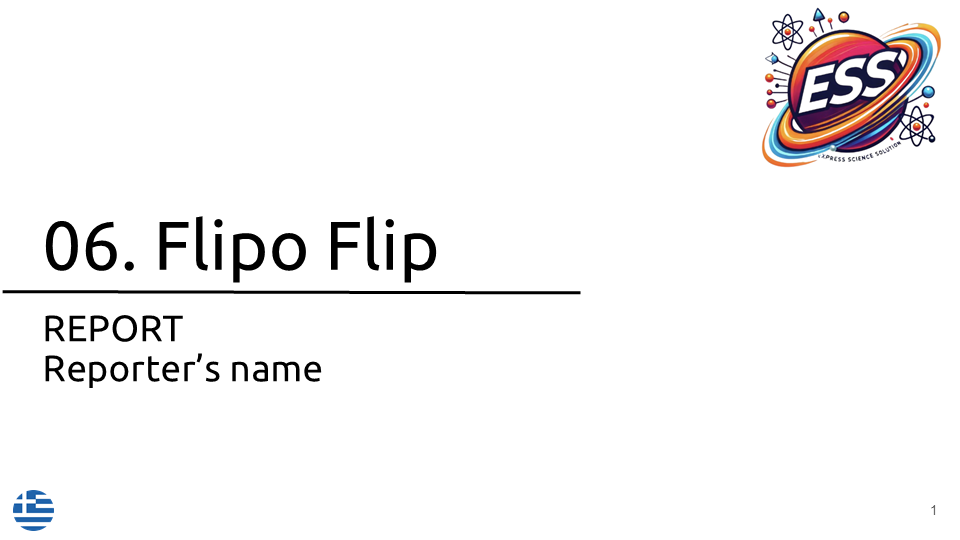
\includegraphics[width=\textwidth]{slides/slide_1.png}
\vspace{0.5em}\noindent\rule{\textwidth}{0.5pt}

Hi, I'm Stelios, and today I will be presenting IYPT 2026 problem \#6: The Flipo Flip.

\clearpage

%% ---- SLIDE 2 ----
\noindent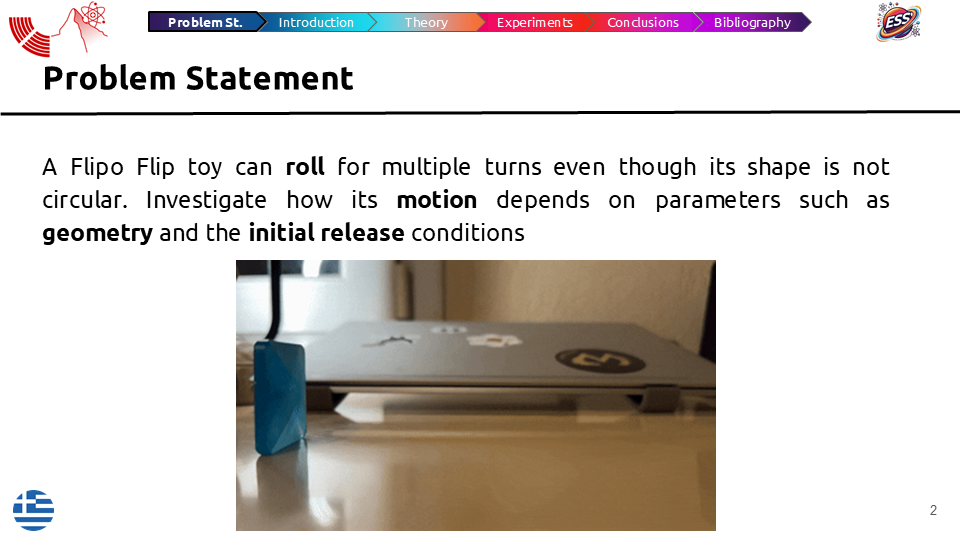
\includegraphics[width=\textwidth]{slides/slide_2.png}
\vspace{0.5em}\noindent\rule{\textwidth}{0.5pt}

The problem statement reads: ``A Flipo Flip toy can roll for multiple turns even though its shape is not circular. Investigate how its motion depends on parameters such as geometry and initial release conditions.'' Our goal in this presentation is to understand the geometry of the toy, develop a theoretical model that connects relevant parameters and describes the motion of the toy, and test our model and assumptions with experimental measurements.

\clearpage

%% ---- SLIDE 3 ----
\noindent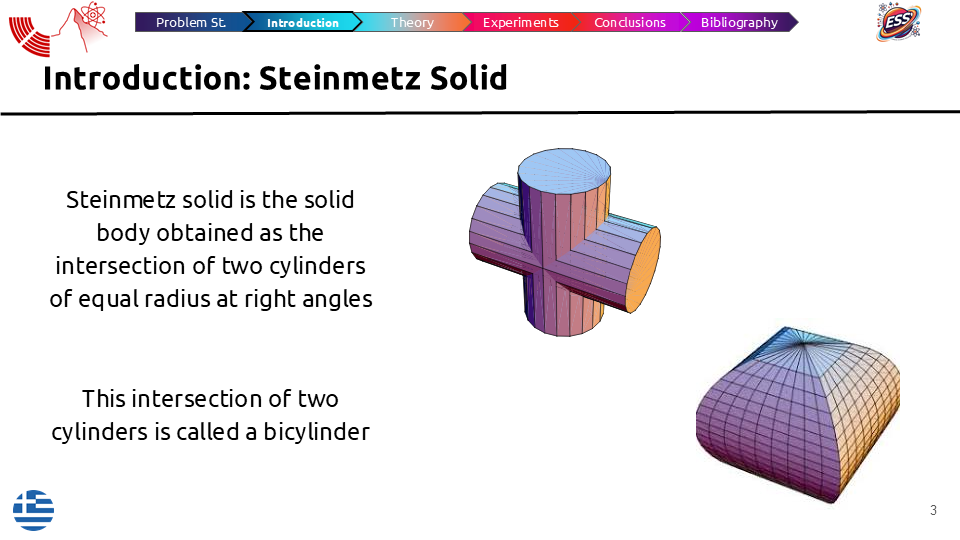
\includegraphics[width=\textwidth]{slides/slide_3.png}
\vspace{0.5em}\noindent\rule{\textwidth}{0.5pt}

Let's start with the geometry of the toy. To understand it, we will use a solid object called the Steinmetz solid, also known as a bicylinder. The Steinmetz solid is the body formed by the intersection of two cylinders of equal radius $R$ at right angles.

\clearpage

%% ---- SLIDE 4 ----
\noindent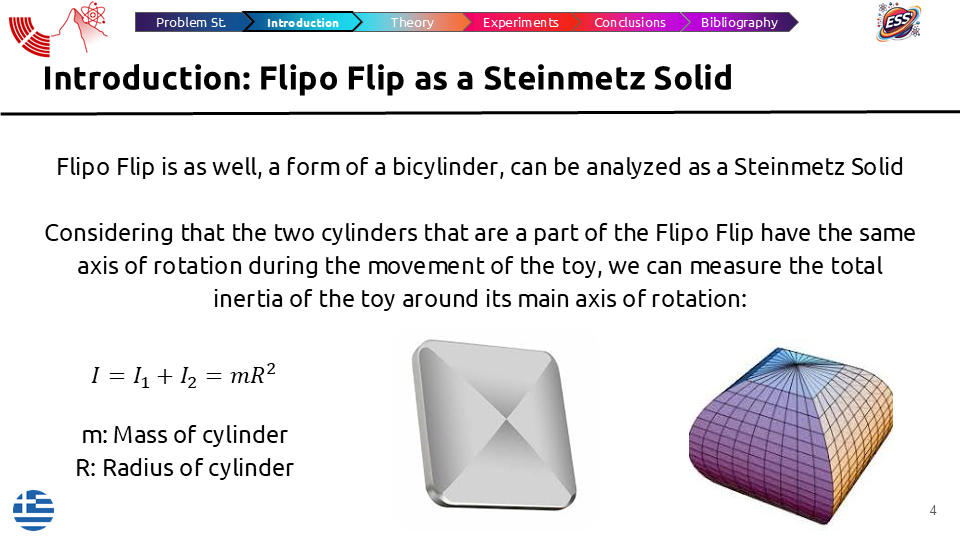
\includegraphics[width=\textwidth]{slides/slide_4.png}
\vspace{0.5em}\noindent\rule{\textwidth}{0.5pt}

The toy is constructed by taking the outer sections of a Steinmetz solid --- the part highlighted here on top, and an identical one from the bottom --- and joining them with a thin square prism with rounded edges. Since both cylinders share the same axis of rotation during the toy's motion, the total moment of inertia about that axis is the sum of the two individual moments of inertia, equal to $mR^2$, where $m$ is the mass of each cylinder and $R$ is its radius. Because this surface comes from a Steinmetz solid, when the toy rolls on it the contact geometry is identical to that of a cylinder of radius $R$ rolling.

\clearpage

%% ---- SLIDE 5 ----
\noindent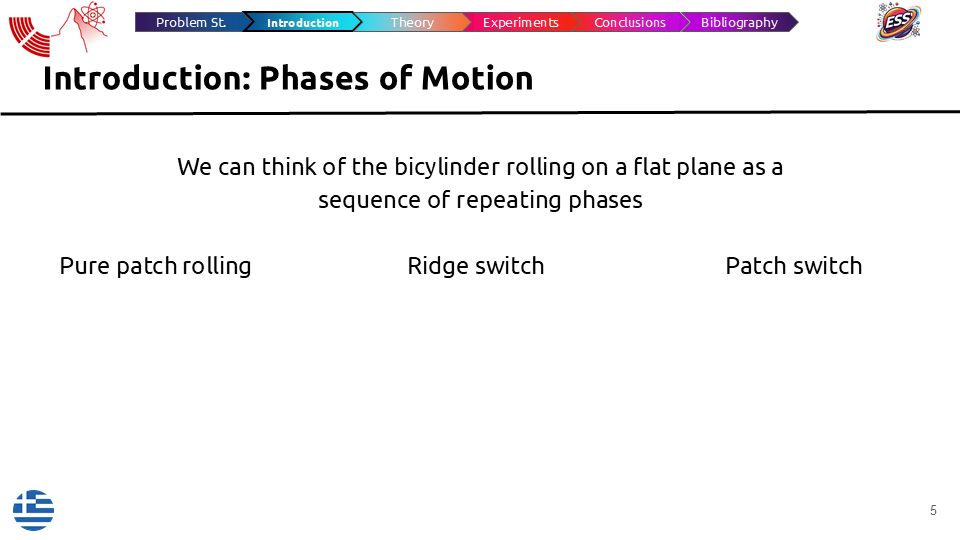
\includegraphics[width=\textwidth]{slides/slide_5.png}
\vspace{0.5em}\noindent\rule{\textwidth}{0.5pt}

Now, let's move on to the categorisation of the phases of motion of the toy. When the toy is rolling on a flat surface, we can describe the motion as a sequence of three repeating phases: Pure patch rolling, Ridge switch, and Patch switch.

\clearpage

%% ---- SLIDE 6 ----
\noindent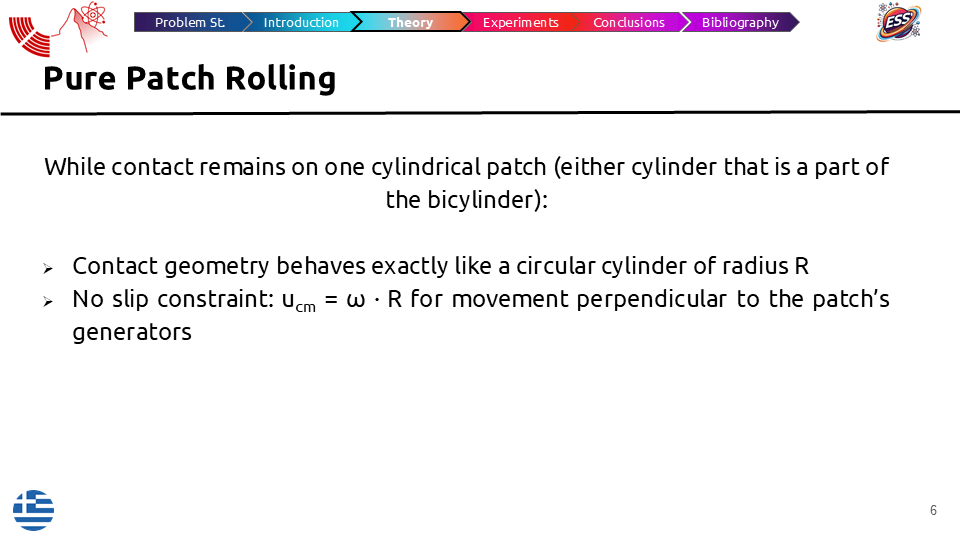
\includegraphics[width=\textwidth]{slides/slide_6.png}
\vspace{0.5em}\noindent\rule{\textwidth}{0.5pt}

Pure patch rolling is the phase in which the toy rolls along its large curved surface --- in other words, when the contact point remains on one cylindrical patch. As I mentioned, during this phase the contact geometry is equivalent to that of a circular cylinder of radius $R$. A key assumption of our model is the no-slip condition: the velocity of the centre of mass equals the angular velocity times the radius --- which is required for rolling to occur.

\clearpage

%% ---- SLIDE 7 ----
\noindent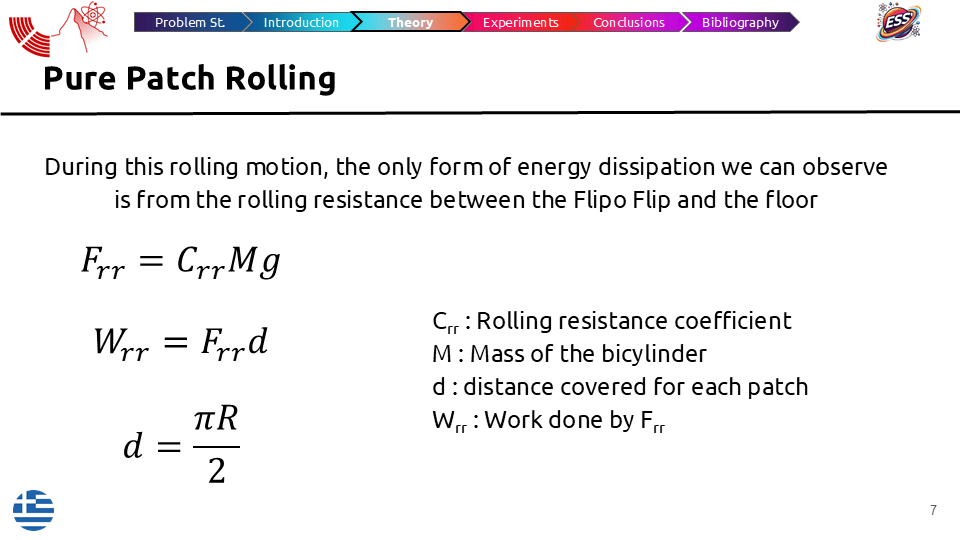
\includegraphics[width=\textwidth]{slides/slide_7.png}
\vspace{0.5em}\noindent\rule{\textwidth}{0.5pt}

During this rolling motion, the only form of energy dissipation we can observe is from the rolling resistance between the Flipo Flip and the floor. The rolling resistance force is equal to the rolling resistance coefficient multiplied by the weight of the bicylinder. The work done by it is the force times the distance travelled during pure patch rolling, and that distance equals $\pi R/2$. Dissipation from aerodynamic drag is negligible given the small velocities the toy achieves. It is also worth noting that rolling resistance only accounts for the dissipation of translational energy; the remaining rotational energy is dissipated by other mechanisms, such as switching dissipation, for the toy to eventually come to rest.

\clearpage

%% ---- SLIDE 8 ----
\noindent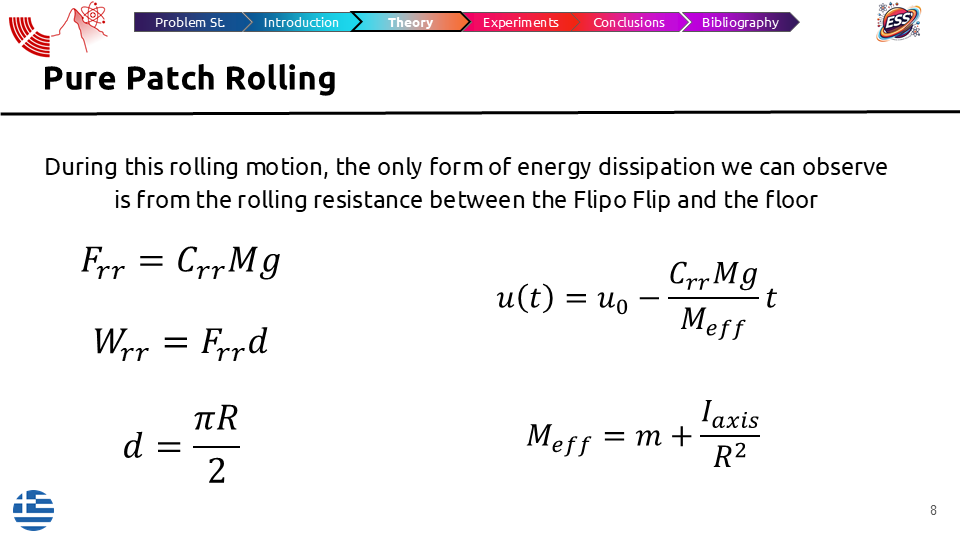
\includegraphics[width=\textwidth]{slides/slide_8.png}
\vspace{0.5em}\noindent\rule{\textwidth}{0.5pt}

Using the rolling resistance force, we can find how the translational velocity $u(t)$ is reduced during pure patch rolling. It equals the initial velocity minus the acceleration multiplied by the time elapsed during pure patch rolling, where the acceleration is the rolling resistance force divided by the effective mass of the toy. The effective mass is the physical mass plus a term related to its rolling inertia.

\clearpage

%% ---- SLIDE 9 ----
\noindent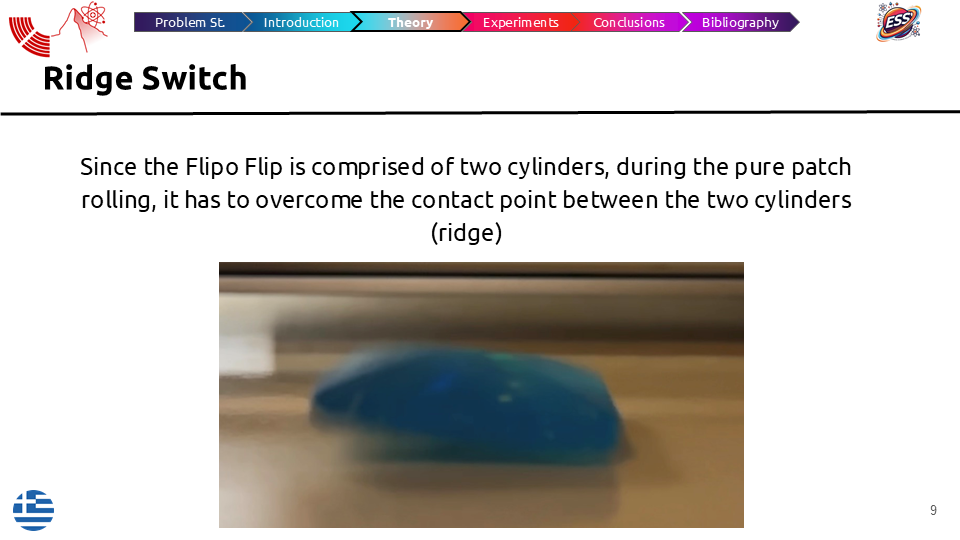
\includegraphics[width=\textwidth]{slides/slide_9.png}
\vspace{0.5em}\noindent\rule{\textwidth}{0.5pt}

Let's move on to the ridge switch. It happens during pure patch rolling, when the contact point passes through the centre of the curved surface --- the contact point between the two cylinders, which we call the ridge. The dissipation and mechanics at this point are already accounted for in pure patch rolling, and nothing changes here; it is just worth noting.

\clearpage

%% ---- SLIDE 10 ----
\noindent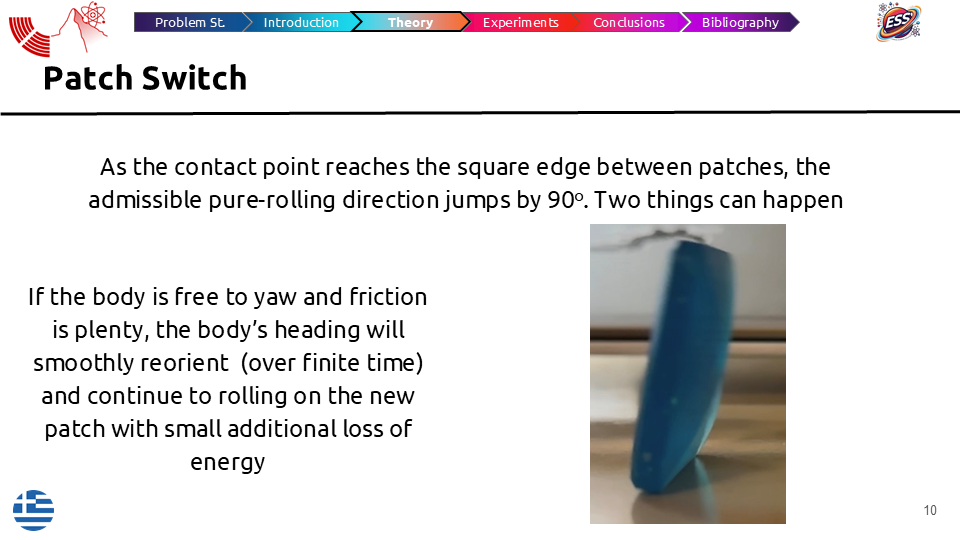
\includegraphics[width=\textwidth]{slides/slide_10.png}
\vspace{0.5em}\noindent\rule{\textwidth}{0.5pt}

The third phase of the motion is the patch switch. During this phase, the contact point is on one of the edges of the square prism at the bottom, or on the entire flat surface --- which occurs only for an instant as it transitions between them. This phase sits between the end of pure patch rolling on one cylindrical patch and the start of pure patch rolling on the other. When the contact point reaches the square edge between patches, the admissible pure-rolling direction jumps by 90 degrees. Two things can happen: if there is sufficient friction, the toy will smoothly reorient over a finite time and continue rolling on the new patch, with some additional energy loss.

\medskip
\noindent\textcolor{gray}{\small\itshape [If asked: The 90-degree change is because the CM velocity was pointing toward the ground, and now it points to the left --- that's 90 degrees.]}

\clearpage

%% ---- SLIDE 11 ----
\noindent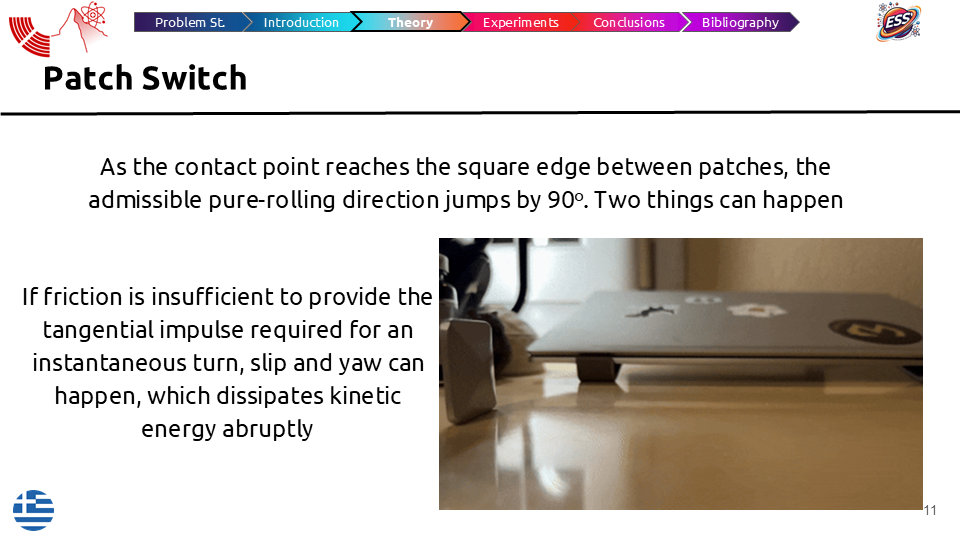
\includegraphics[width=\textwidth]{slides/slide_11.png}
\vspace{0.5em}\noindent\rule{\textwidth}{0.5pt}

But if friction is insufficient to provide the tangential impulse required for an instantaneous turn, the toy will slip and yaw, which dissipates energy quickly and prevents any additional flips.

\clearpage

%% ---- SLIDE 12 ----
\noindent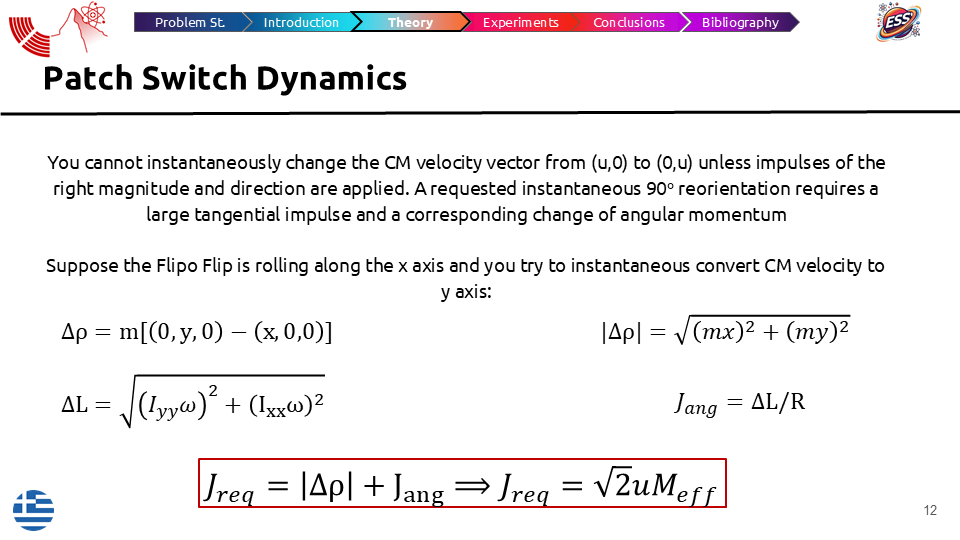
\includegraphics[width=\textwidth]{slides/slide_12.png}
\vspace{0.5em}\noindent\rule{\textwidth}{0.5pt}

You cannot instantaneously change the CM velocity vector from $(u,0)$ to $(0,u)$ --- the 90-degree change I've been referring to --- unless impulses of the right magnitude and direction are applied. An instantaneous 90-degree reorientation requires a large tangential impulse and a corresponding change in angular momentum. To quantify this, suppose the Flipo Flip is rolling along the $x$-axis and we want to redirect its CM velocity to the $y$-axis. We only care about the magnitude of the change, which is why we chose two orientations differing by 90 degrees. We start with the change in momentum, which is mass times the difference of the CM velocity vectors for a 90-degree change. From this we find the magnitude of that change: the square root of the sum of squares of the initial and final momenta. We then find the change in angular momentum as the square root of the sum of squares of the initial and final angular momenta --- each equal to their respective moment of inertia times angular velocity. Converting the change in angular momentum to the required impulse by dividing by $R$, and summing with the translational impulse, gives us the total required impulse $J_{\mathrm{req}}$, which works out to $\sqrt{2}$ times velocity times the effective mass.

\clearpage

%% ---- SLIDE 13 ----
\noindent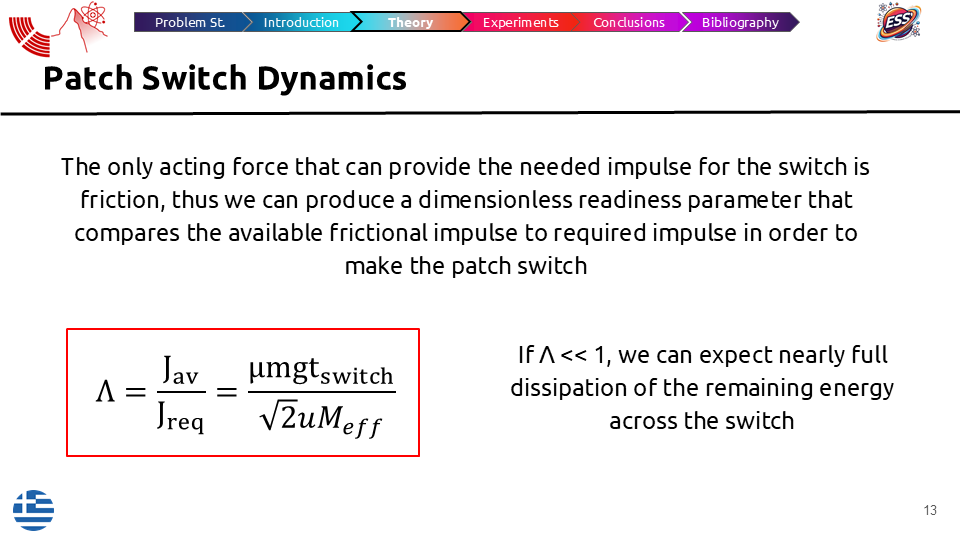
\includegraphics[width=\textwidth]{slides/slide_13.png}
\vspace{0.5em}\noindent\rule{\textwidth}{0.5pt}

The only force that can provide this impulse is friction. We can therefore define a dimensionless number $\Lambda$ (Lambda) that compares the available frictional impulse to the required impulse for the patch switch. If $\Lambda$ is much smaller than one, most of the energy will be lost during the switch and the motion will stop there. Generally, $\Lambda$ is between 0 and 1, and it controls how much energy is dissipated during each patch switch.

\clearpage

%% ---- SLIDE 14 ----
\noindent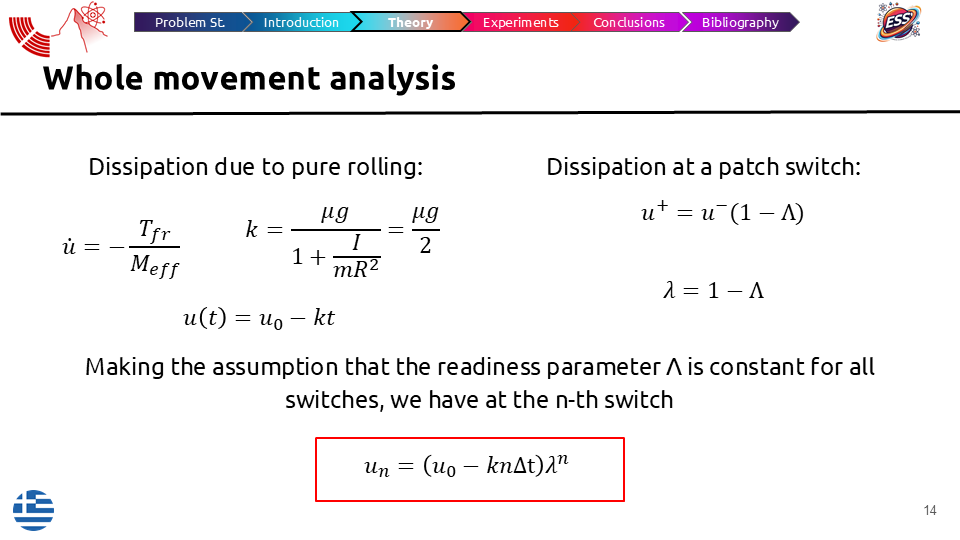
\includegraphics[width=\textwidth]{slides/slide_14.png}
\vspace{0.5em}\noindent\rule{\textwidth}{0.5pt}

Let's move on to the full motion analysis. We have the equations derived for pure patch rolling, now rewritten, alongside the patch switch dissipation equations. For pure patch rolling, the acceleration equals minus the friction force divided by the effective mass, which equals $k$, and after some calculations equals the rolling friction coefficient times $g$ over 2. We also have the function that describes how velocity decreases during pure rolling. For patch switch dissipation, the velocity right after the patch switch equals the velocity before the switch times $(1 - \Lambda)$. This is how $\Lambda$ controls energy dissipation at each patch switch. If we assume $\Lambda$ is constant across all switches, we can write an expression for the velocity at the $n$-th switch, accounting for all preceding patch switches and rolling phases.

\clearpage

%% ---- SLIDE 15 ----
\noindent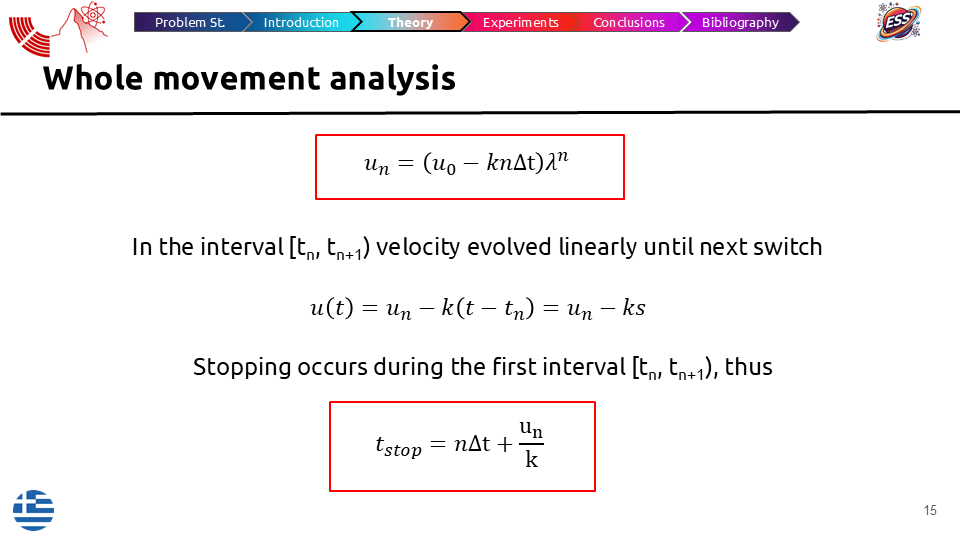
\includegraphics[width=\textwidth]{slides/slide_15.png}
\vspace{0.5em}\noindent\rule{\textwidth}{0.5pt}

In each pure patch rolling interval, velocity evolves linearly, and is then multiplied by a factor less than one at each patch switch. Velocity can only reach zero during the linear decrease, not during the proportional drop of a patch switch, and from this we get the equation for $t_{\mathrm{stop}}$ --- the time at which the Flipo Flip stops rolling.

\clearpage

%% ---- SLIDE 16 ----
\noindent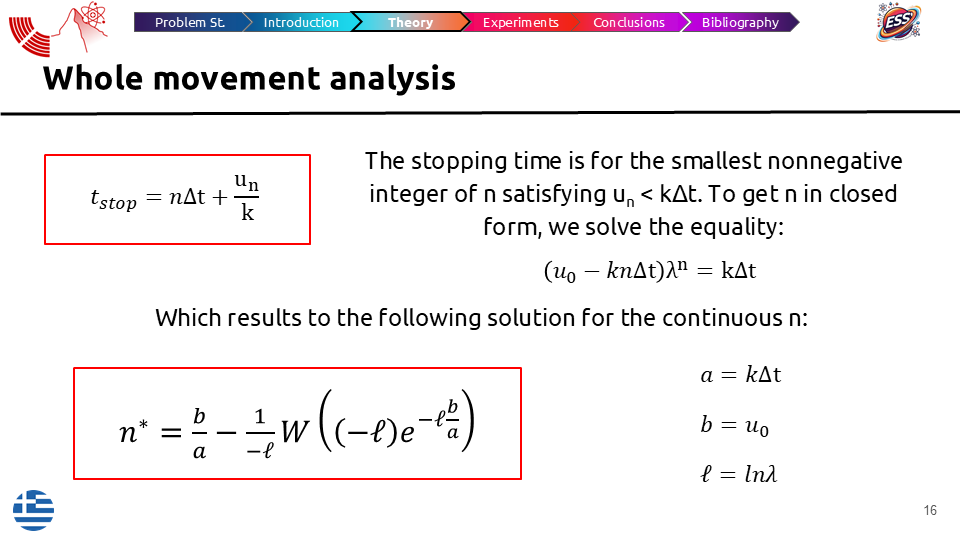
\includegraphics[width=\textwidth]{slides/slide_16.png}
\vspace{0.5em}\noindent\rule{\textwidth}{0.5pt}

The toy stops at the smallest nonnegative integer $n$ satisfying $u_n < k\Delta t$. To get $n$ in closed form, we solve the equality, which gives the following expression for continuous $n$.

\clearpage

%% ---- SLIDE 17 ----
\noindent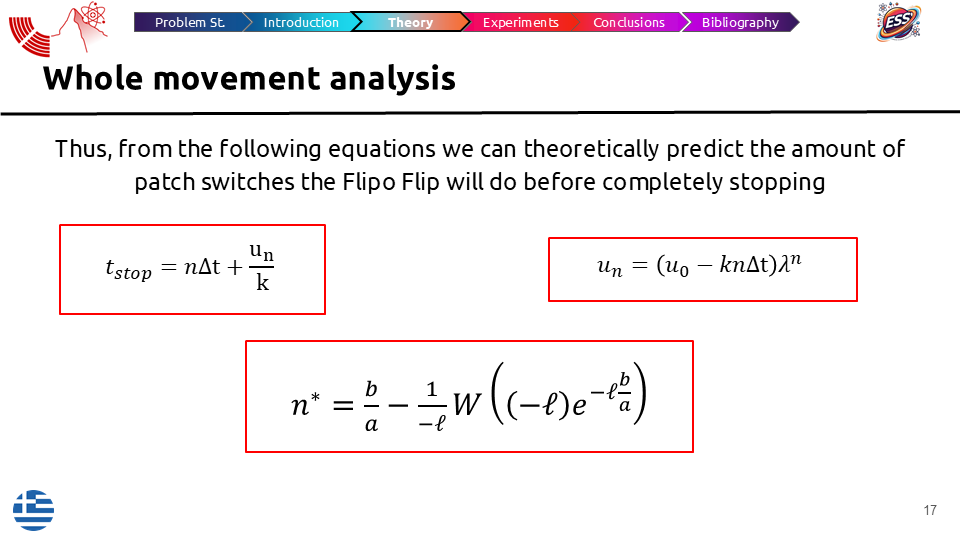
\includegraphics[width=\textwidth]{slides/slide_17.png}
\vspace{0.5em}\noindent\rule{\textwidth}{0.5pt}

These are the equations I have described, and from them we can theoretically predict the number of patch switches the Flipo Flip will make before stopping. These are the equations used for the theoretical predictions in the plots you will see in the experiments section.

\clearpage

%% ---- SLIDE 18 ----
\noindent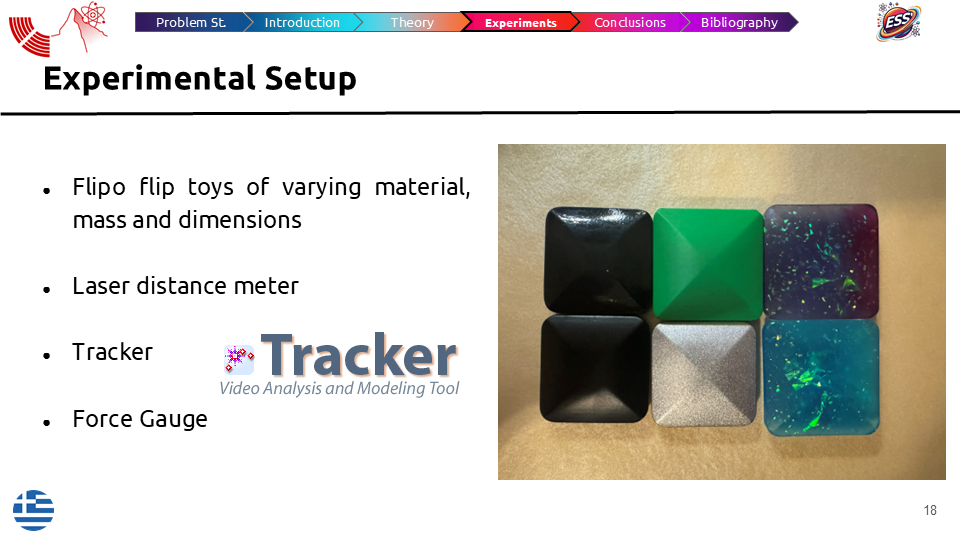
\includegraphics[width=\textwidth]{slides/slide_18.png}
\vspace{0.5em}\noindent\rule{\textwidth}{0.5pt}

Now that we have completed the theoretical model, let's move on to our experiments. For our setup, we used 6 Flipo Flips with different materials, masses, and dimensions, a laser distance meter, Tracker video analysis software, and a force gauge to apply different forces to the toy.

\clearpage

%% ---- SLIDE 19 ----
\noindent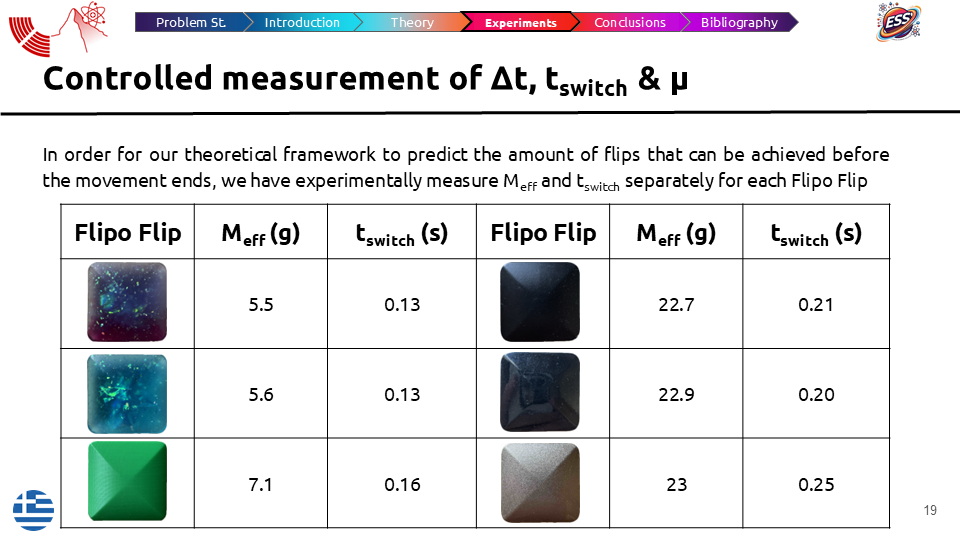
\includegraphics[width=\textwidth]{slides/slide_19.png}
\vspace{0.5em}\noindent\rule{\textwidth}{0.5pt}

In order for our theoretical model to predict the number of flips before motion stops, we experimentally measured the effective mass, the patch switch time, and the rolling friction coefficient separately for each Flipo Flip.

\clearpage

%% ---- SLIDE 20 ----
\noindent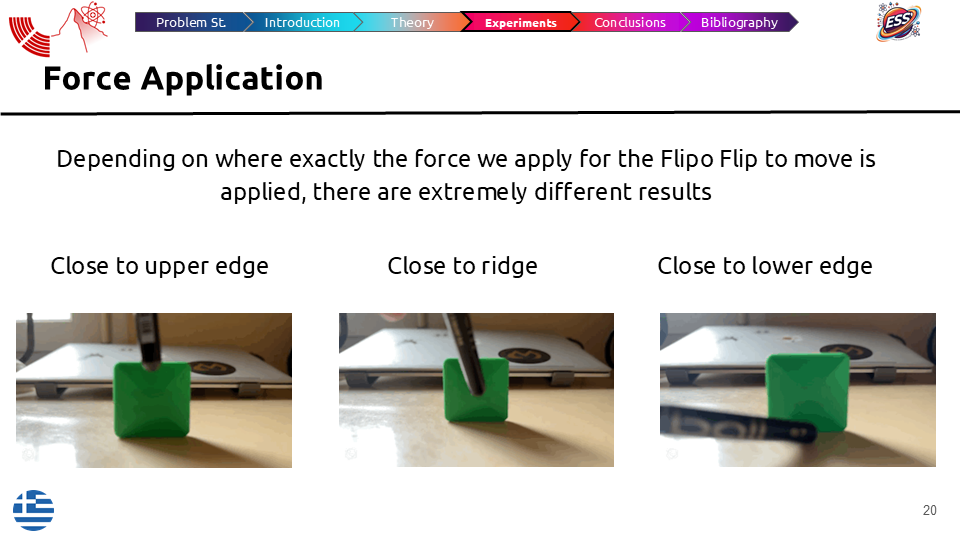
\includegraphics[width=\textwidth]{slides/slide_20.png}
\vspace{0.5em}\noindent\rule{\textwidth}{0.5pt}

The first part of our analysis has to do with force application. We measured the number of flips the toy could do before slipping or stopping as a function of initial velocity, but how that velocity is applied matters. We may apply a force in any of the visible locations,

\clearpage

%% ---- SLIDE 21 ----
\noindent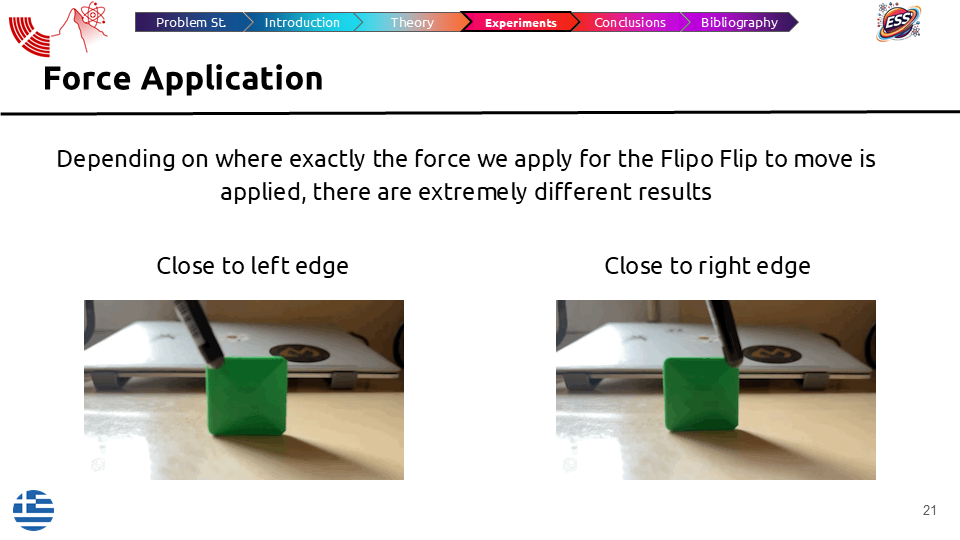
\includegraphics[width=\textwidth]{slides/slide_21.png}
\vspace{0.5em}\noindent\rule{\textwidth}{0.5pt}

and only some of them will initiate the motion.

\clearpage

%% ---- SLIDE 22 ----
\noindent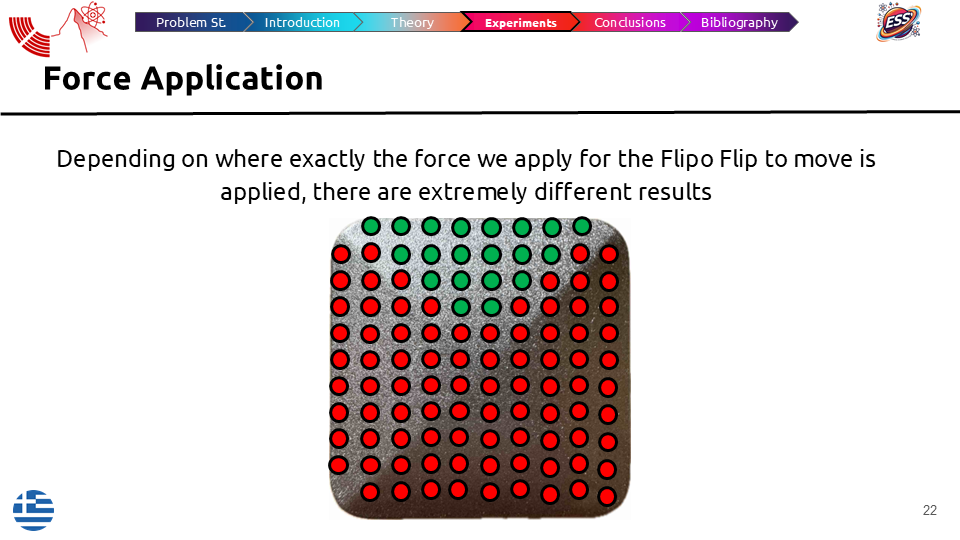
\includegraphics[width=\textwidth]{slides/slide_22.png}
\vspace{0.5em}\noindent\rule{\textwidth}{0.5pt}

Here, we can see all the locations the initial force was applied during our experiments, but only the green ones actually allowed the motion to start.

\clearpage

%% ---- SLIDE 23 ----
\noindent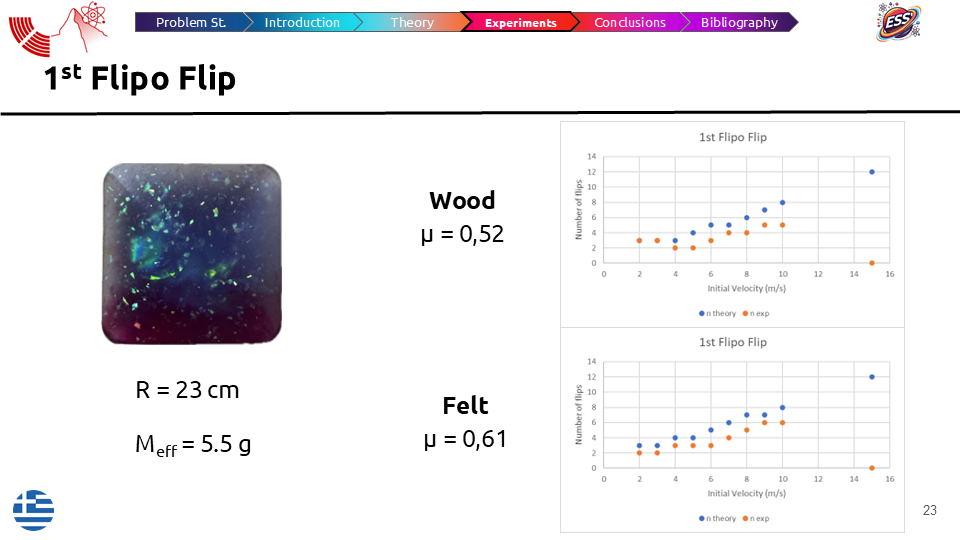
\includegraphics[width=\textwidth]{slides/slide_23.png}
\vspace{0.5em}\noindent\rule{\textwidth}{0.5pt}

For each of the 6 Flipo Flips, the experiment went as follows: the Flipo Flip was placed upright, and a force was applied to the centre of the surface above the ridge using the force gauge. We used that force to give the toy an initial velocity, measured with Tracker. We then recorded the number of flips for each initial velocity, producing the (initial velocity, number of flips) pairs visible on the diagram. This process was repeated until ten such pairs were obtained. Each Flipo Flip has 10 data points for each of two different surfaces --- in other words, 20 experimental values per Flipo Flip, ten on one surface type and ten on another, in order to vary the rolling friction coefficient. We used integer initial velocities from 2~m/s up to 10~m/s, plus 15~m/s. Here you can see the two graphs corresponding to the two surfaces for each Flipo Flip, with their experimentally measured friction coefficients, and a plot of the experimental and theoretical data points.

\clearpage

%% ---- SLIDE 24 ----
\noindent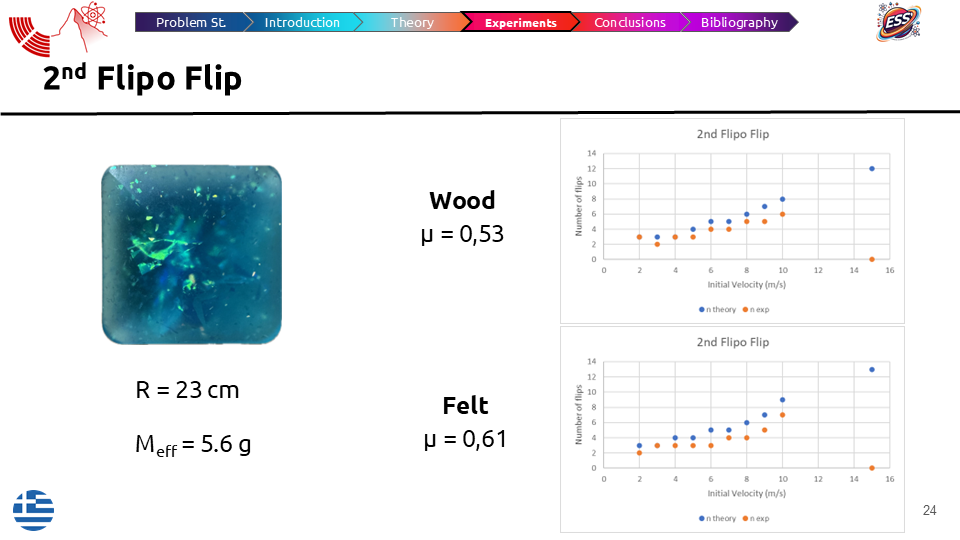
\includegraphics[width=\textwidth]{slides/slide_24.png}
\vspace{0.5em}\noindent\rule{\textwidth}{0.5pt}

Our model generally overpredicts or matches the number of flips observed in each experiment. This is likely because of additional losses not captured in the model, such as air resistance or minor deformations. Another contributing factor is the simplifying assumptions we made: we keep $\Lambda$ constant, whereas in practice it would decrease, and we treat $t_{\mathrm{switch}}$ as constant, whereas it would increase as the velocity drops --- each patch switch taking longer and therefore dissipating more energy. The no-slip assumption also plays a role: since we assume the toy never slips, it may slip earlier than its available energy would otherwise permit, which produces the gap between the theoretical and experimental data.

\clearpage

%% ---- SLIDE 25 ----
\noindent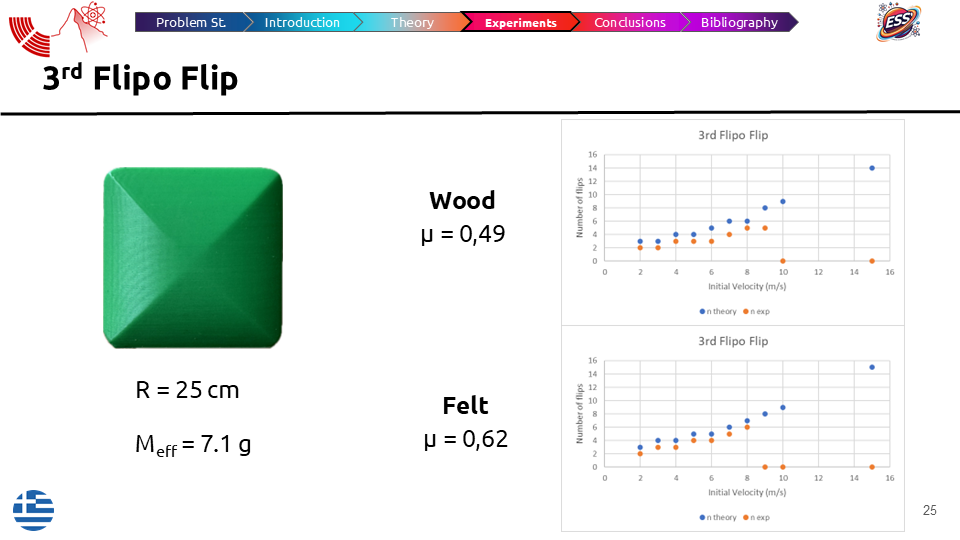
\includegraphics[width=\textwidth]{slides/slide_25.png}
\vspace{0.5em}\noindent\rule{\textwidth}{0.5pt}

We can also see that there is a critical velocity for each Flipo Flip, above which the toy does no flips at all, while the model predicts an increasing number. We will discuss that shortly.

\clearpage

%% ---- SLIDE 26 ----
\noindent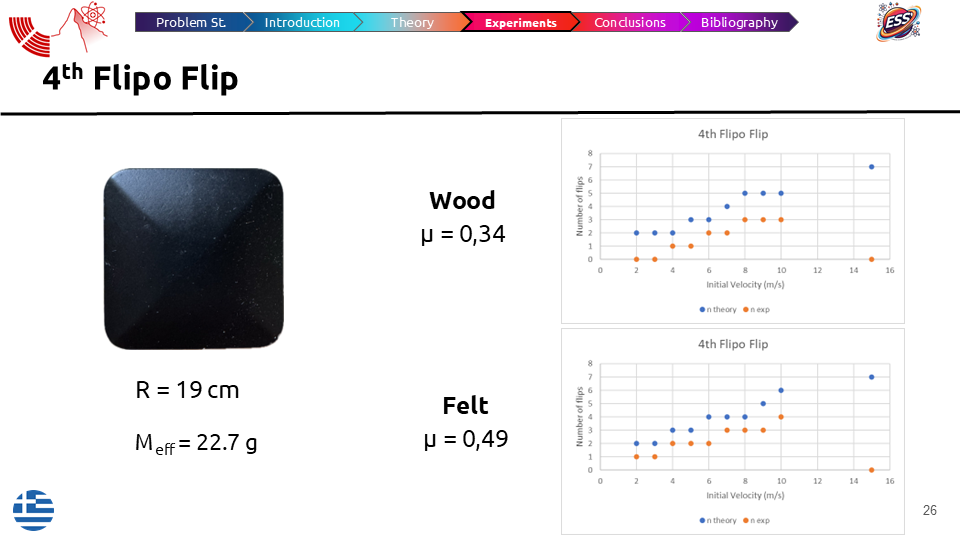
\includegraphics[width=\textwidth]{slides/slide_26.png}
\vspace{0.5em}\noindent\rule{\textwidth}{0.5pt}

We can also see that a smaller friction coefficient leads to a larger error in our model. We believe this is related to the no-slip assumption: when the rolling friction coefficient is smaller, the toy is more likely to slip before it would otherwise stop based on its available energy alone.

\clearpage

%% ---- SLIDE 27 ----
\noindent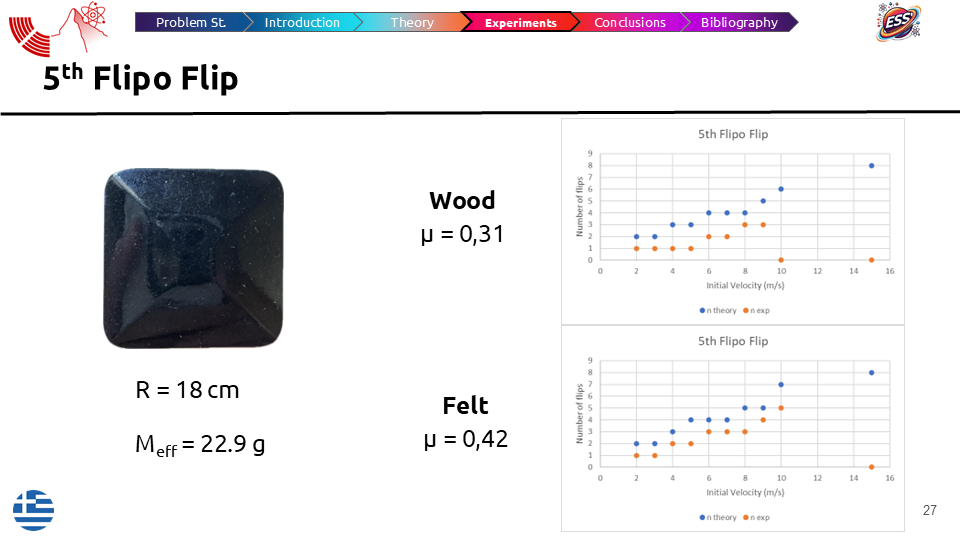
\includegraphics[width=\textwidth]{slides/slide_27.png}
\vspace{0.5em}\noindent\rule{\textwidth}{0.5pt}

As you can see, the trends we discussed are consistent across all the Flipo Flips.

\clearpage

%% ---- SLIDE 28 ----
\noindent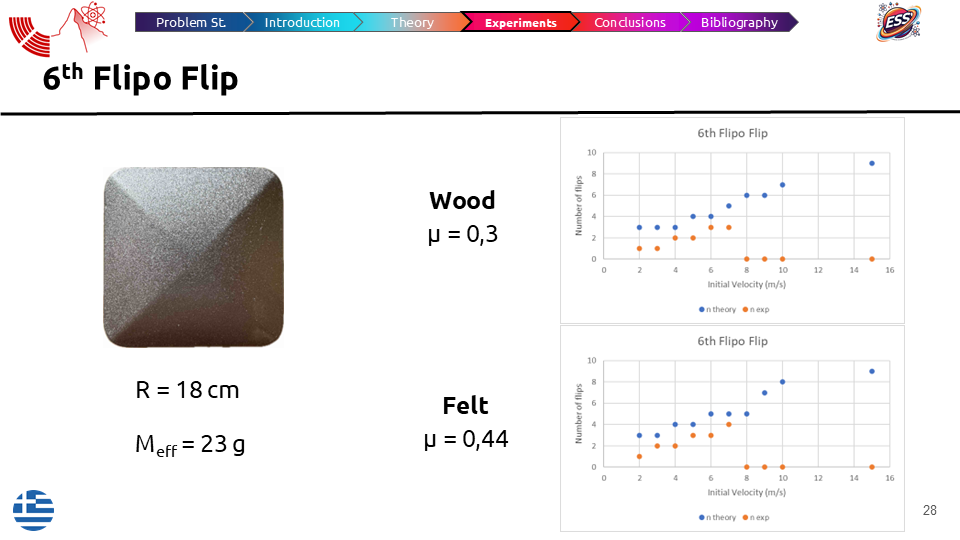
\includegraphics[width=\textwidth]{slides/slide_28.png}
\vspace{0.5em}\noindent\rule{\textwidth}{0.5pt}

And this is our last Flipo Flip, which also has the smallest critical velocity. Time to address the elephant in the room.

\clearpage

%% ---- SLIDE 29 ----
\noindent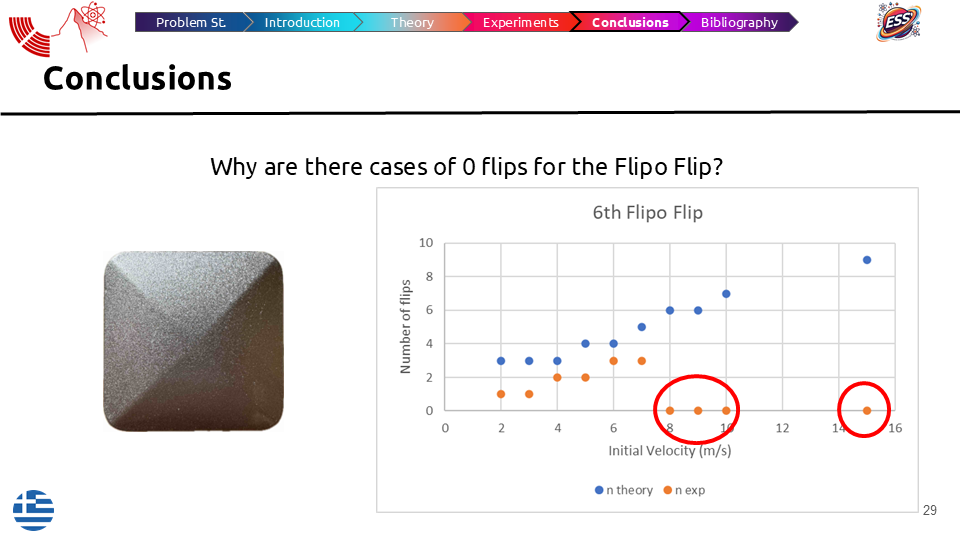
\includegraphics[width=\textwidth]{slides/slide_29.png}
\vspace{0.5em}\noindent\rule{\textwidth}{0.5pt}

Why are there cases where 0 flips are done? In other words, why does a critical velocity exist? It's also due to the no-slip condition.

\clearpage

%% ---- SLIDE 30 ----
\noindent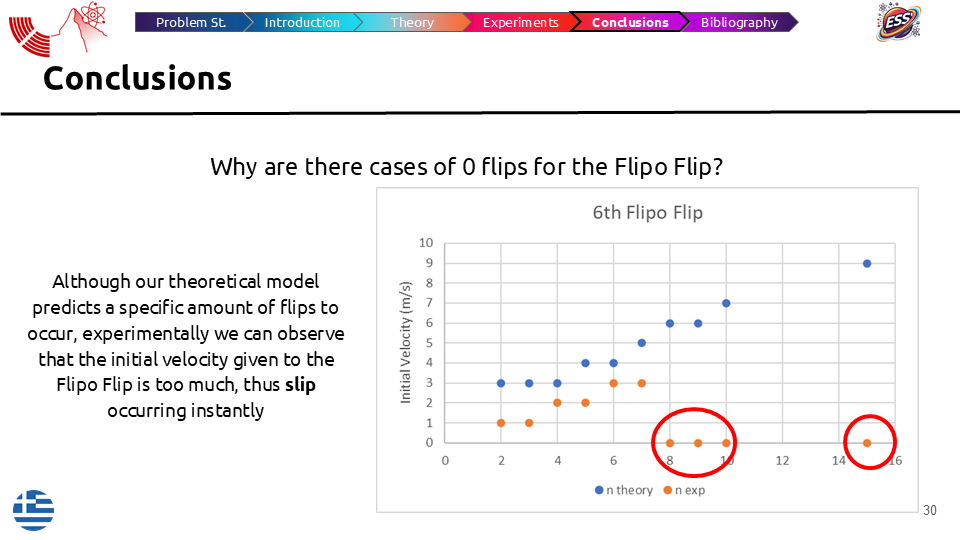
\includegraphics[width=\textwidth]{slides/slide_30.png}
\vspace{0.5em}\noindent\rule{\textwidth}{0.5pt}

To model the toy's motion, we assumed it actually rolls. But sometimes the no-slip condition cannot hold from the very start, because the initial velocity is too high for the toy to maintain ground contact, and it gets launched into the air.

\clearpage

%% ---- SLIDE 31 ----
\noindent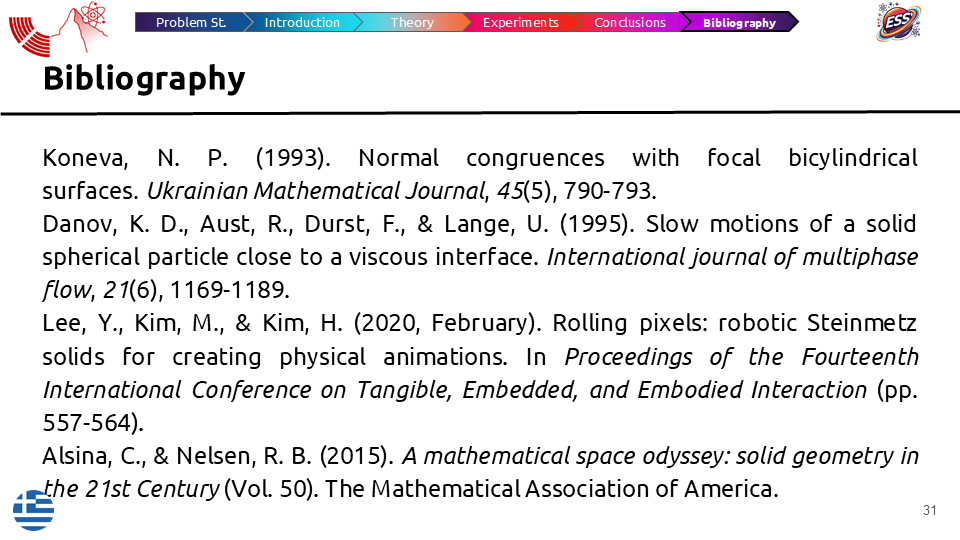
\includegraphics[width=\textwidth]{slides/slide_31.png}
\vspace{0.5em}\noindent\rule{\textwidth}{0.5pt}

Here's our bibliography.

\clearpage

%% ---- SLIDE 32 ----
\noindent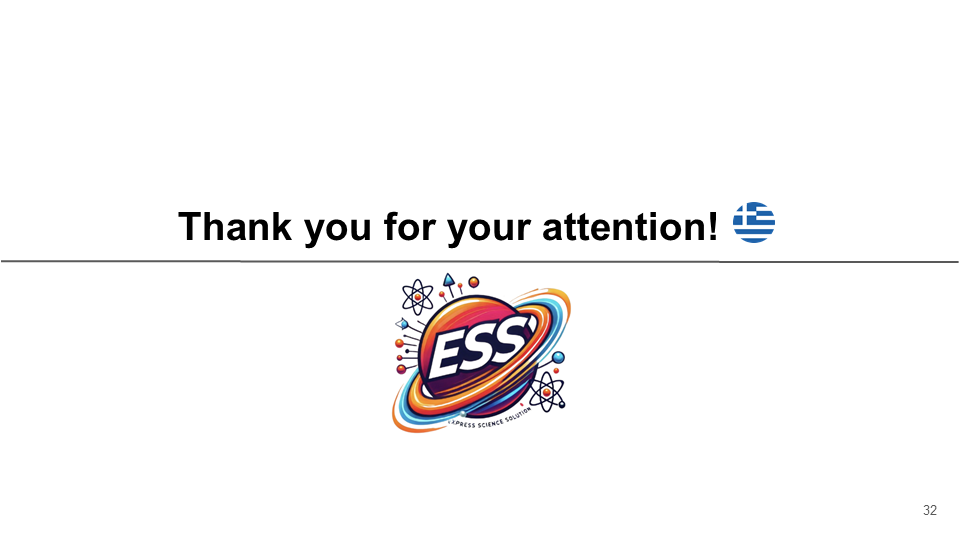
\includegraphics[width=\textwidth]{slides/slide_32.png}
\vspace{0.5em}\noindent\rule{\textwidth}{0.5pt}

And thank you very much for your attention!

\clearpage

%% ---- SLIDE 33 ----
\noindent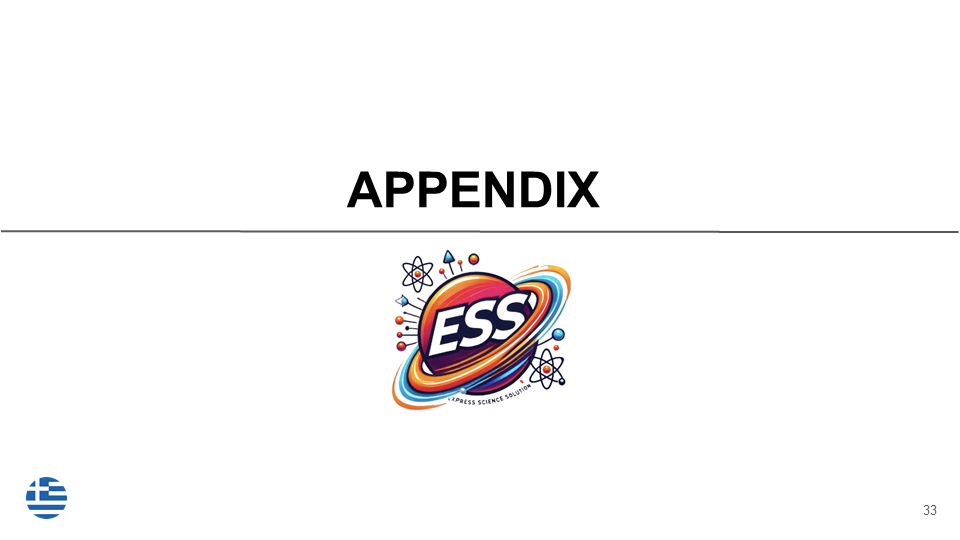
\includegraphics[width=\textwidth]{slides/slide_33.png}
\vspace{0.5em}\noindent\rule{\textwidth}{0.5pt}

\textit{No spoken text.}

\end{document}
